% TeleCon Classic Simple — code guide for the Arduino sketch.
% Build: pdflatex -output-directory=../build telecon_classic_simple_code.tex
% Delivered PDF: ../build/telecon_classic_simple_code.pdf
\documentclass[11pt,a4paper]{article}

\usepackage[margin=2.2cm]{geometry}
\usepackage[T1]{fontenc}
\usepackage[utf8]{inputenc}
\usepackage{lmodern}
\usepackage{booktabs}
\usepackage{hyperref}
\usepackage{xcolor}
\usepackage{colortbl}
\usepackage{array}
\usepackage{enumitem}
\usepackage{needspace}
\usepackage{etoolbox}
\usepackage{fancyvrb}
\usepackage{tikz}
\usetikzlibrary{arrows.meta,positioning,shapes.geometric,fit,backgrounds}

\preto\section{\Needspace{8\baselineskip}}

\hypersetup{
  colorlinks=true,
  linkcolor=black,
  urlcolor=blue,
  pdfhighlight=/N,
  pdftitle={TeleCon Classic Simple code guide},
  pdfauthor={TeleCon}
}

\definecolor{TblHead}{HTML}{0F6F73}
\definecolor{TblChan}{HTML}{D5F5E3}
\definecolor{TblEdit}{HTML}{F5CBA7}
\definecolor{TblTelem}{HTML}{D4E6F1}
\definecolor{TblLeave}{HTML}{F4F6F7}

\newcommand{\thc}[1]{\textcolor{white}{\bfseries #1}}
\newcommand{\chip}[2]{\colorbox{#1}{\strut\,\scriptsize #2\,}}
\newcommand{\ui}[1]{\textsf{\textbf{#1}}}
\newcommand{\code}[1]{\texttt{#1}}

\newcommand{\sketchfile}{../../../ESP32_noCam/Classic_Simple/TeleCon_Classic_Simple/TeleCon_Classic_Simple.ino}
\newcommand{\channelfile}{../../../ESP32_noCam/Classic_Simple/TeleCon_Classic_Simple/TelemetryChannels.h}

\newcommand{\inosnippet}[2]{%
  \VerbatimInput[%
    firstline=#1,lastline=#2,%
    numbers=left,firstnumber=#1,%
    fontsize=\footnotesize,%
    frame=single,framerule=0.4pt,rulecolor=\color{TblHead},%
    xleftmargin=1.8em%
  ]{\sketchfile}%
}
\newcommand{\hsnippet}[2]{%
  \VerbatimInput[%
    firstline=#1,lastline=#2,%
    numbers=left,firstnumber=#1,%
    fontsize=\footnotesize,%
    frame=single,framerule=0.4pt,rulecolor=\color{TblHead},%
    xleftmargin=1.8em%
  ]{\channelfile}%
}

\tikzset{
  flow/.style={draw=TblHead, fill=TblChan, rounded corners=2pt,
               align=center, font=\sffamily\small, inner sep=5pt,
               minimum height=8mm},
  edit/.style={draw=TblHead, fill=TblEdit, rounded corners=2pt,
               align=center, font=\sffamily\small\bfseries, inner sep=5pt},
  leave/.style={draw=TblHead!70, fill=TblLeave, rounded corners=2pt,
                align=center, font=\sffamily\small, inner sep=5pt},
  arr/.style={-{Stealth[length=2.2mm]}, draw=TblHead, thick}
}

\title{Classic + Simple\\[0.25em]
\large Code guide for \texttt{TeleCon\_Classic\_Simple}}
\author{ESP32 DevKit \textperiodcentered\ Bluetooth Classic \textperiodcentered\ text lines}
\date{Version 1.0 \quad 2026}

\begin{document}
\maketitle

\begin{abstract}
This note is the Arduino sketch
\texttt{ESP32\_noCam/Classic\_Simple/TeleCon\_Classic\_Simple/}.
The phone setting is Classic + Simple. The board name is
\texttt{ESP32-TC-RC-BT-Simple}. The handshake is
\texttt{RC:CONNECT,proto,simple}. The pages below show every file the
IDE compiles, how one session runs, and the three places a vehicle
sketch is supposed to change: \texttt{onControl()}, \texttt{onButton()},
and \texttt{kTelemetryChannels[]}.
\end{abstract}

{\sffamily\scriptsize
\chip{TblEdit}{Change this}
\chip{TblChan}{Already working}
\chip{TblLeave}{Leave it alone}}

\tableofcontents
\vspace{0.6em}

\section{The folder Arduino opens}

Open the folder that contains the \texttt{.ino}. The IDE compiles every
source in that folder. \texttt{README.md} is not compiled.

\begin{center}
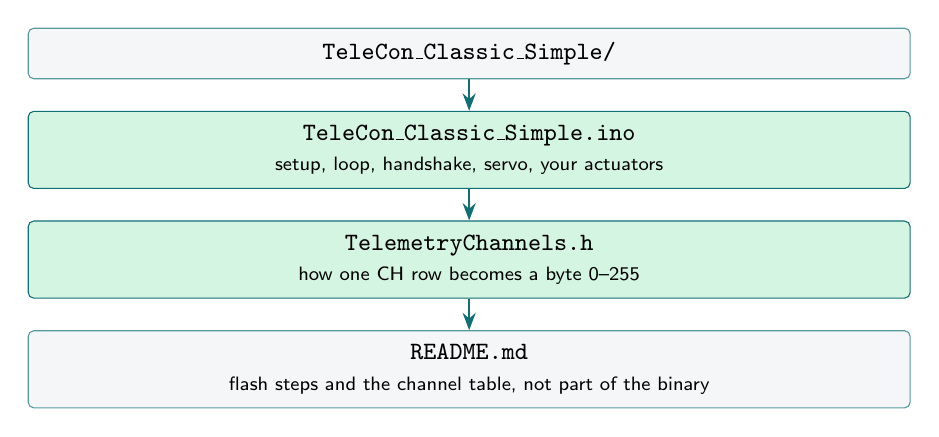
\begin{tikzpicture}[node distance=4mm]
  \node[leave, minimum width=11.2cm] (dir) {\texttt{TeleCon\_Classic\_Simple/}};
  \node[flow, below=of dir, minimum width=11.2cm] (ino)
    {\texttt{TeleCon\_Classic\_Simple.ino}\\
     \scriptsize setup, loop, handshake, servo, your actuators};
  \node[flow, below=of ino, minimum width=11.2cm] (h)
    {\texttt{TelemetryChannels.h}\\
     \scriptsize how one CH row becomes a byte 0--255};
  \node[leave, below=of h, minimum width=11.2cm] (md)
    {\texttt{README.md}\\
     \scriptsize flash steps and the channel table, not part of the binary};
  \draw[arr] (dir) -- (ino);
  \draw[arr] (ino) -- (h);
  \draw[arr] (h) -- (md);
\end{tikzpicture}
\end{center}

Board in the Arduino IDE: \ui{ESP32 Dev Module}. Serial Monitor:
115200~baud, line ending Newline. In the phone: Board DevKit, connection
Classic + Simple. Pair \texttt{ESP32-TC-RC-BT-Simple}. If Android asks
for a PIN, it is \texttt{1234}.

Do not copy this sketch onto an ESP32-CAM. Video uses the
video-only sketch on a second board. Sticks stay on this Bluetooth link.

\section{One session, from pair to plot}
\label{sec:session}

Nothing in \texttt{onControl()} runs until the phone has completed the
handshake. Telemetry is the same: \texttt{loop()} returns early while
\texttt{handshakeOk} is false.

\begin{center}
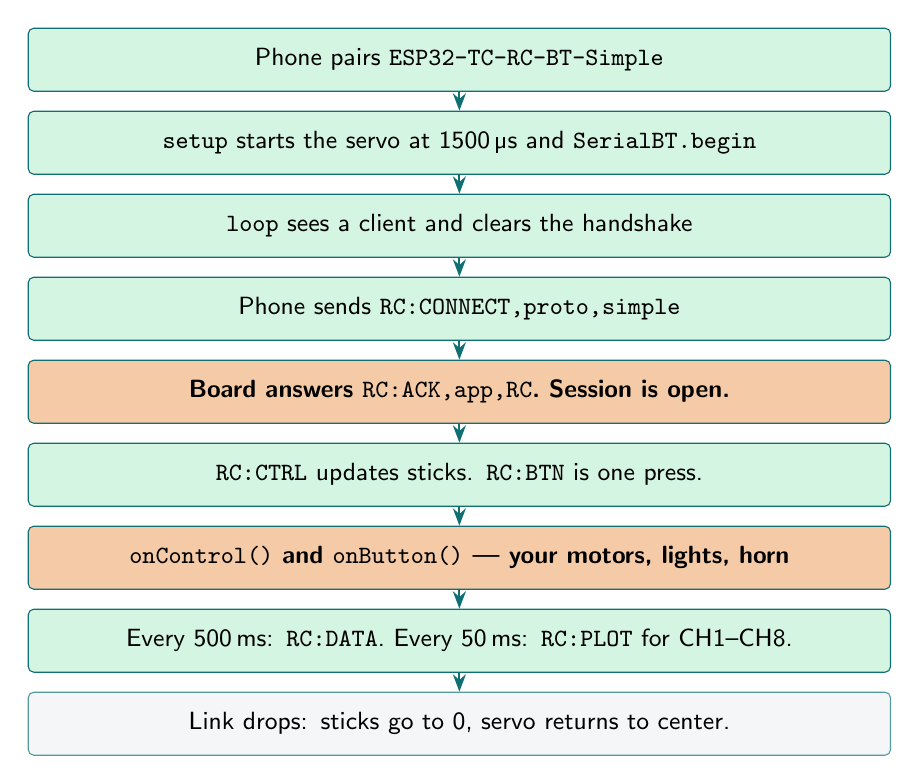
\begin{tikzpicture}[
  node distance=2.4mm,
  every node/.style={flow, text width=10.6cm}
]
  \node (a) {Phone pairs \texttt{ESP32-TC-RC-BT-Simple}};
  \node[below=of a] (b) {\texttt{setup} starts the servo at 1500\,\textmu s and \texttt{SerialBT.begin}};
  \node[below=of b] (c) {\texttt{loop} sees a client and clears the handshake};
  \node[below=of c] (d) {Phone sends \texttt{RC:CONNECT,proto,simple}};
  \node[edit, below=of d, text width=10.6cm] (e) {Board answers \texttt{RC:ACK,app,RC}. Session is open.};
  \node[below=of e] (f) {\texttt{RC:CTRL} updates sticks. \texttt{RC:BTN} is one press.};
  \node[edit, below=of f, text width=10.6cm] (g) {\texttt{onControl()} and \texttt{onButton()} --- your motors, lights, horn};
  \node[below=of g] (h) {Every 500\,ms: \texttt{RC:DATA}. Every 50\,ms: \texttt{RC:PLOT} for CH1--CH8.};
  \node[leave, below=of h, text width=10.6cm] (i) {Link drops: sticks go to 0, servo returns to center.};
  \draw[arr] (a) -- (b);
  \draw[arr] (b) -- (c);
  \draw[arr] (c) -- (d);
  \draw[arr] (d) -- (e);
  \draw[arr] (e) -- (f);
  \draw[arr] (f) -- (g);
  \draw[arr] (g) -- (h);
  \draw[arr] (h) -- (i);
\end{tikzpicture}
\end{center}

\section{Where to change the sketch}
\label{sec:edit}

Most of the file is the link. A vehicle project only needs the orange
rows. Leave the parser, the Bluetooth name, and \texttt{proto,simple}
alone unless you are deliberately making a different product. The phone
matches this sketch by that name and that handshake.

\begin{center}
\renewcommand{\arraystretch}{1.22}
\setlength{\tabcolsep}{4pt}
\begin{tabular}{>{\raggedright\arraybackslash}p{4.4cm}
                >{\raggedright\arraybackslash}p{5.6cm}
                >{\raggedright\arraybackslash}p{5.0cm}}
\rowcolor{TblHead}
\thc{You want} & \thc{Edit} & \thc{Leave} \\
\rowcolor{TblEdit}
Drive motors, a second servo, lights & \texttt{onControl()}, the block marked \texttt{YOUR CODE HERE} & \texttt{handleLine()}, \texttt{getValue()} \\
\rowcolor{TblEdit}
Horn, pan-center, extra buttons & \texttt{onButton()} & Button ids the phone already sends \\
\rowcolor{TblEdit}
Stop motors when Bluetooth drops & \texttt{applyFailSafe()}, the second \texttt{YOUR CODE HERE} & The stick reset above that comment \\
\rowcolor{TblEdit}
What CH1--CH8 show on the phone & \texttt{kTelemetryChannels[]} in the \texttt{.ino} & Do not add a ninth row \\
\rowcolor{TblEdit}
Real temperature or battery & \texttt{telemetryVehicle()}, cases \texttt{TEL\_TEMP} and \texttt{TEL\_BATT}, or change that row to \texttt{TEL\_ADC} & The 0--255 range \\
\rowcolor{TblEdit}
Servo on another pin, or no servo & \texttt{PIN\_STEER\_SERVO}, or \texttt{ENABLE\_STEER\_SERVO} set to 0 & \texttt{rx = 0} means 1500\,\textmu s \\
\rowcolor{TblChan}
Quiet Serial Monitor & \texttt{ENABLE\_DEBUG}, \texttt{ENABLE\_PLOT}, \texttt{ENABLE\_SERIAL\_INJECT} set to 0 & Flash again after the change \\
\rowcolor{TblLeave}
A different phone protocol & Do not retarget this file & Use Classic Binary or BLE Binary \\
\end{tabular}
\end{center}

\texttt{rx} is already shifted by the phone trim before it arrives.
This sketch does not store a steering center. Do not add a
\texttt{RC:SET,steer\_center} handler.

\section{Name, pin, and switches}
\label{sec:config}

\inosnippet{16}{45}

\texttt{BT\_NAME} and \texttt{BT\_PIN} are what Android sees while
pairing. \texttt{APP\_PREFIX} and \texttt{PROTO\_WIRE} are what
\texttt{handleConnect()} accepts. If either string changes, the phone
setting Classic + Simple will get \texttt{RC:NAK} and
\texttt{onControl()} will never run.

\texttt{ENABLE\_DEBUG} turns the \texttt{DBG\_*} macros into
\texttt{Serial.print}, or into nothing. The session still runs when
they are empty. \texttt{ENABLE\_PLOT} is the 50\,ms \texttt{RC:PLOT}
stream. \texttt{ENABLE\_SERIAL\_INJECT} lets you paste one
\texttt{RC:DATA} or \texttt{RC:PLOT} line into the Serial Monitor after
the handshake; the next automatic packet replaces it.
\texttt{DEMO\_MOTOR\_TEMP} and \texttt{DEMO\_BATT\_PCT} are the stand-in
HUD numbers until a sensor is wired. They are not read from a pin.

\section{What the sketch remembers}

\inosnippet{47}{70}

One \texttt{RC:CTRL} line fills the six controls and the switch byte.
Until the first line arrives, sticks are 0 and both knobs are 512
(mid-scale of 0--1023). \texttt{handshakeOk} is the gate in
\texttt{loop()} and in \texttt{handleLine()}. \texttt{btWasConnected}
exists only so a connect or a drop is noticed once, not on every pass
of \texttt{loop()}.

The \texttt{lastPrint*} variables belong to the Serial Monitor. They
are not sent to the phone. A stick is printed only when its 12-bit
image changes, so a resting stick does not flood the monitor.

\begin{center}
\renewcommand{\arraystretch}{1.15}
\setlength{\tabcolsep}{4pt}
\begin{tabular}{ll>{\raggedright\arraybackslash}p{8.2cm}}
\rowcolor{TblHead}
\thc{Name} & \thc{Range} & \thc{Phone control} \\
\rowcolor{TblChan}
\texttt{g\_lx}, \texttt{g\_ly} & $-100$ \ldots\ $100$ & Left stick X, left stick Y (throttle) \\
\rowcolor{TblChan}
\texttt{g\_rx}, \texttt{g\_ry} & $-100$ \ldots\ $100$ & Right stick X (steering), right stick Y \\
\rowcolor{TblChan}
\texttt{g\_lk}, \texttt{g\_rk} & $0$ \ldots\ $1023$ & Left knob, right knob. 512 is the middle. \\
\rowcolor{TblChan}
\texttt{g\_sw} & 8 bits, sent as hex & Bit 0 is the lights switch. Bits 1--5 are the other switches. \\
\end{tabular}
\end{center}

\section{CH1 to CH8}
\label{sec:channels}

The phone has eight plot channels and no ninth. Row 0 of the table is
CH1, which the wire calls \texttt{v0}. Row 7 is CH8, \texttt{v7}.
Each sample is one byte, 0--255.

\inosnippet{100}{114}

The header file defines the row and the readers. The \texttt{.ino}
only fills the table and answers the built-in signals.

\hsnippet{17}{42}

\begin{center}
\renewcommand{\arraystretch}{1.18}
\setlength{\tabcolsep}{3pt}
\begin{tabular}{>{\raggedright\arraybackslash}p{2.3cm}
                >{\raggedright\arraybackslash}p{4.4cm}
                >{\raggedright\arraybackslash}p{7.6cm}}
\rowcolor{TblHead}
\thc{Kind} & \thc{Fields that matter} & \thc{Byte that is sent} \\
\rowcolor{TblTelem}
\texttt{TEL\_VEHICLE} & \texttt{vehicle} & \texttt{telemetryVehicle()} in the \texttt{.ino}. \texttt{pin} is ignored. \\
\rowcolor{TblTelem}
\texttt{TEL\_ADC} & \texttt{pin} & \texttt{analogRead}, 0--4095 scaled to 0--255. Use a GPIO that can be an input, such as 34 or 35. \\
\rowcolor{TblTelem}
\texttt{TEL\_GPIO} & \texttt{pin} & \texttt{digitalRead}: 0 or 255. An output pin reports the level last written. \\
\rowcolor{TblTelem}
\texttt{TEL\_PWM} & \texttt{pin}, \texttt{ledcChannel}, \texttt{dutyMin}, \texttt{dutyMax} & LEDC duty already running on that pin. \texttt{dutyMin} becomes 0 and \texttt{dutyMax} becomes 255. \\
\end{tabular}
\end{center}

Stock rows, top to bottom:

\begin{center}
\renewcommand{\arraystretch}{1.12}
\setlength{\tabcolsep}{4pt}
\begin{tabular}{>{\raggedright\arraybackslash}p{1.6cm}
                >{\raggedright\arraybackslash}p{1.5cm}
                >{\raggedright\arraybackslash}p{11.2cm}}
\rowcolor{TblHead}
\thc{Phone} & \thc{Wire} & \thc{Stock source} \\
\rowcolor{TblChan}
CH1 & \texttt{v0} & Demo temperature, constant 90 \\
CH2 & \texttt{v1} & Throttle magnitude $|$\texttt{g\_ly}$|$. Direction is not in the byte. \\
CH3 & \texttt{v2} & Demo battery 76\%, scaled to 0--255 \\
CH4 & \texttt{v3} & Steering magnitude $|$\texttt{g\_rx}$|$ \\
CH5 & \texttt{v4} & Lights, switch bit 0, as 0 or 255 \\
CH6 & \texttt{v5} & Left knob, 0--1023 scaled to 0--255 \\
CH7 & \texttt{v6} & Right knob, same scale \\
CH8 & \texttt{v7} & Steering-servo PWM. Duty 204\ldots409 is the 1000--2000\,\textmu s travel. Center is about 128. \\
\end{tabular}
\end{center}

\inosnippet{116}{137}

\texttt{TEL\_RY} is implemented and unused by the stock table. To show
the right-stick Y axis, replace a row's \texttt{vehicle} with
\texttt{TEL\_RY}. Throttle, steer, and \texttt{TEL\_RY} are magnitudes:
full left and full right are the same byte. A signed axis needs a
center of 128, for example
\code{map(g\_ly, -100, 100, 0, 255)}, written in
\texttt{telemetryVehicle()} for that one signal.

A real battery on GPIO 34 replaces the CH3 row. The vehicle name on an
ADC row is ignored:

\begin{quote}
\texttt{\{ TEL\_ADC, TEL\_BATT, 34, -1, 0, 1 \},}
\end{quote}

An 8-bit motor PWM on GPIO 25, LEDC channel 0, is:

\begin{quote}
\texttt{\{ TEL\_PWM, TEL\_THROTTLE, 25, 0, 0, 255 \},}
\end{quote}

The pin must already be attached with \texttt{ledcAttach} (Arduino-ESP32
3.x) or \texttt{ledcSetup} plus \texttt{ledcAttachPin} (2.x) before the
plot reads it. The reader itself is in the header and is the same for
every row.

\hsnippet{46}{75}

On core 3.x, \texttt{ledcRead} takes the GPIO number. On 2.x it takes
the channel number. That is why a PWM row stores both \texttt{pin} and
\texttt{ledcChannel}.

Changing a row does not add packets. The plot line is still eight
numbers every 50\,ms, about 80 bytes, about 1.6\,kB/s. The phone channel
menus bind CH1--CH8. There is nowhere to put a CH9.

\section{Steering servo}

\inosnippet{87}{176}

The servo is on by default, GPIO 13, LEDC channel 2, 50\,Hz, 12-bit
duty. \texttt{rx = 0} is 1500\,\textmu s. Full stick is $\pm 500$\,\textmu s,
so the pulse runs from 1000\,\textmu s to 2000\,\textmu s. The duty is
$\mathrm{pulse} \times 4095 / 20000$, because a 20\,ms frame at 12 bits
is 4096 steps.

\begin{center}
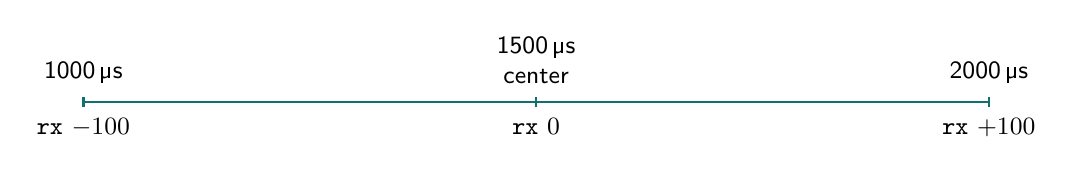
\begin{tikzpicture}[x=1.15cm,y=0.55cm]
  \draw[TblHead, thick] (0,0) -- (10,0);
  \foreach \x/\lab in {0/$-100$,5/$0$,10/$+100$}{
    \draw[TblHead, thick] (\x,-0.12) -- (\x,0.12);
    \node[below, font=\sffamily\small] at (\x,-0.15) {\texttt{rx} \lab};
  }
  \node[above, font=\sffamily\small, align=center] at (0,0.2) {1000\,\textmu s};
  \node[above, font=\sffamily\small, align=center] at (5,0.2) {1500\,\textmu s\\center};
  \node[above, font=\sffamily\small, align=center] at (10,0.2) {2000\,\textmu s};
\end{tikzpicture}
\end{center}

Phone trim already moves \texttt{rx} before this function sees it.
\texttt{steerServoWriteRx(0)} in the fail-safe is center, not ``whatever
trim was last''.

To move the servo to another pin, change \texttt{PIN\_STEER\_SERVO}.
Keep \texttt{CH\_STEER\_SERVO} off the channels you later use for motor
PWM (the binary sketches use 0 and 1 for the two drive motors, 2 for
steer, 3 for pan). To build a board with no servo, set
\texttt{ENABLE\_STEER\_SERVO} to 0. The two functions become empty, and
CH8 will read 0 because no PWM is attached.

Core 3.x writes the LEDC channel by pin number. Core 2.x writes it by
channel number. Both branches are in \texttt{steerServoBegin()} and
\texttt{steerServoWriteRx()}.

\section{Your actuators}
\label{sec:yourcode}

\inosnippet{178}{198}

\texttt{onControl()} runs once per \texttt{RC:CTRL} line, which the
phone sends many times a second while a stick is held. Put continuous
outputs here: motor PWM, a pan servo from \texttt{rk}, a lights pin from
\texttt{sw \& 0x01}. The steering call above the comment is already
done. The \texttt{(void)} casts only silence unused-parameter warnings;
delete a cast when you start using that value.

\texttt{onButton()} runs once per press. The phone button id is the
argument. The stock comments reserve id 2 for a short horn pulse and
id 4 for centering a pan servo. Those bodies are empty on purpose.
A button that must stay down for the whole hold is a better fit as a
switch bit in \texttt{onControl()}, because \texttt{RC:BTN} is an edge,
not a level.

\inosnippet{409}{416}

On disconnect, sticks, knobs, and switches return to the same defaults
as boot, and the servo is written to center. Motor PWM you started in
\texttt{onControl()} is \emph{not} cleared unless you stop it under the
second \texttt{YOUR CODE HERE}. A driver left at the last throttle will
keep running after the phone is gone.

\section{setup}

\inosnippet{200}{242}

Order matters. Serial starts first so a Bluetooth failure can be
printed. The servo is centered before the radio comes up, so a link
that never connects still leaves the wheel straight.
\texttt{disableSSP()} plus \texttt{setPin(..., 4)} is legacy PIN
pairing. Mixing that with Secure Simple Pairing is a known way to make
Android fail the bond, which is why SSP is turned off.
\texttt{SerialBT.begin(name, false, true)} means ``not the master'' and
``Classic only, BLE off''. If \texttt{begin} fails, the sketch stops in
\texttt{while (true)}.

The banner is entirely debug. It does not change the protocol. It
prints the lines you can paste into the Serial Monitor when inject is
on.

\section{loop}

\inosnippet{244}{302}

Each pass does four things, in this order.

\begin{enumerate}[leftmargin=1.3cm]
  \item Watch the Classic client. A new client clears the handshake so
        an old session cannot stay ``ready'' across a reconnect. A drop
        calls \texttt{applyFailSafe()}.
  \item Read every complete line from Bluetooth and hand it to
        \texttt{handleLine()}. The delimiter is \texttt{\textbackslash n}.
        A line with no characters after \texttt{trim} is ignored.
  \item If inject is compiled in, take one newline-terminated line from
        the Serial Monitor.
  \item If the handshake is still open, return. No \texttt{RC:DATA} and
        no \texttt{RC:PLOT} until \texttt{RC:ACK} has been sent.
\end{enumerate}

After the gate, two timers run from \texttt{millis()}. They do not
reset each other.

\texttt{RC:DATA} every 500\,ms is the vehicle HUD, not the eight plot
channels. \texttt{left} is $|$\texttt{g\_ly}$| \times 2.5$, sent as an
integer (\texttt{abs(g\_ly) * 25 / 10}): full throttle 100 becomes 250,
which the phone treats as speed $\times 10$. \texttt{right} is always
0 in this starter. \texttt{lo,1,ro,0,lg,1,rg,0} are fixed panel lamps.
\texttt{analog} is the demo temperature, \texttt{batt} the demo
percentage, \texttt{led} the switch byte in two hex digits. Replace
\texttt{analog} and \texttt{batt} in this \texttt{snprintf} when the
HUD should follow the same sensor as CH1 or CH3. The plot table does
not fill this line by itself.

\texttt{RC:PLOT} every 50\,ms calls \texttt{telemetryReadAll}, which
walks the eight rows. The line is always
\texttt{v0} through \texttt{v7}, in that order.

\section{Handshake and the text parser}
\label{sec:parser}

\inosnippet{425}{508}

\texttt{getValue()} understands one shape:
\texttt{RC:TYPE,key,value,key,value}. It skips the
\texttt{APP:TYPE} head, then walks pairs. The value runs to the next
comma, or to the end of the line for the last pair. Keys are case
sensitive (\texttt{lx}, not \texttt{LX}). A missing key returns an
empty string, and \texttt{toInt()} of that string is 0, so a broken
\texttt{RC:CTRL} looks like centered sticks.

\texttt{handleConnect()} checks two things. The app name before the
colon must be \texttt{RC}. The \texttt{proto} value must be
\texttt{simple}. Anything else is \texttt{RC:NAK} with
\texttt{app\_mismatch} or \texttt{proto\_mismatch}, and
\texttt{handshakeOk} stays false. Success is exactly
\texttt{RC:ACK,app,RC}.

\texttt{handleLine()} ignores a line with no colon. \texttt{CONNECT}
is accepted before the session is ready; every other type is dropped
until then. After the ACK, only an \texttt{RC} app is accepted.
\texttt{CTRL} stores the seven fields and calls \texttt{onControl()}.
\texttt{BTN} reads \texttt{id} and calls \texttt{onButton()}. Any other
type (\texttt{DATA}, \texttt{PLOT}, \texttt{SET}) is ignored on the
way in. This sketch sends \texttt{DATA} and \texttt{PLOT}; it does not
obey them.

\begin{center}
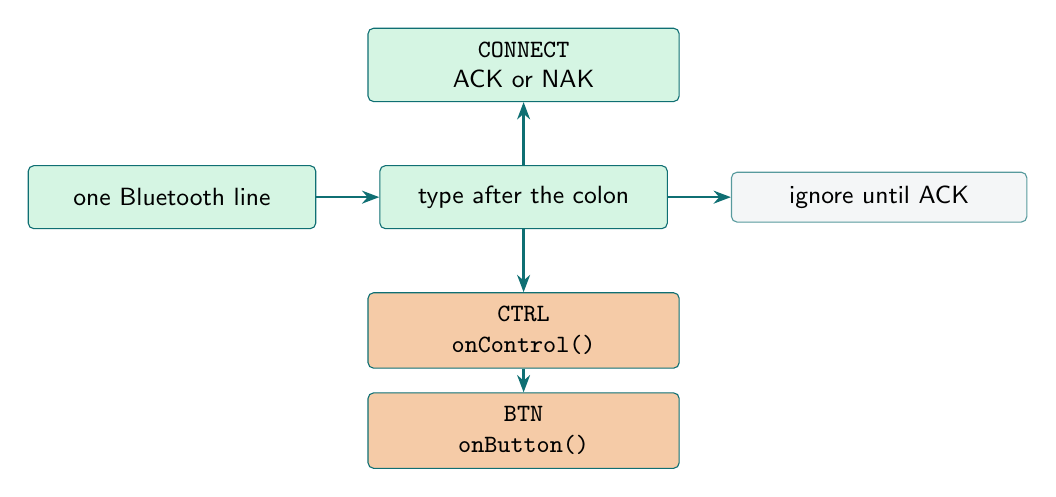
\begin{tikzpicture}[node distance=3mm]
  \node[flow, text width=3.3cm] (line) {one Bluetooth line};
  \node[flow, right=8mm of line, text width=3.3cm] (type) {type after the colon};
  \node[leave, right=8mm of type, text width=3.4cm] (drop) {ignore until ACK};
  \node[edit, below=8mm of type, text width=3.6cm] (ctrl) {\texttt{CTRL}\\\texttt{onControl()}};
  \node[edit, below=of ctrl, text width=3.6cm] (btn) {\texttt{BTN}\\\texttt{onButton()}};
  \node[flow, above=8mm of type, text width=3.6cm] (con) {\texttt{CONNECT}\\ACK or NAK};
  \draw[arr] (line) -- (type);
  \draw[arr] (type) -- (con);
  \draw[arr] (type) -- (ctrl);
  \draw[arr] (ctrl) -- (btn);
  \draw[arr] (type) -- (drop);
\end{tikzpicture}
\end{center}

\section{Serial inject and the monitor}

\inosnippet{304}{347}

Inject is a bench tool. It does not run when Bluetooth has no client,
and it does not run before the handshake. Only a line that starts with
\texttt{RC:DATA} or \texttt{RC:PLOT} is written to the phone, once.
The 500\,ms and 50\,ms timers are not stopped, so the following
automatic line overwrites that inject on the phone. A line longer than
192 characters is thrown away. \texttt{\textbackslash r} is stripped so
a monitor set to ``Both NL \& CR'' still works; the sketch commits on
\texttt{\textbackslash n}.

\inosnippet{349}{402}

\texttt{stickTo12()} maps $-100\ldots100$ onto $0\ldots4095$ for the
monitor only. 0 on the stick is about 2048 on this scale. That number
is not the servo duty and not the plot byte. \texttt{debugPrintControl()}
prints a stick when that axis changes.
It prints \texttt{SW1}--\texttt{SW6} when a bit flips. \texttt{debugPrintButton()} prints the
id. With \texttt{ENABLE\_DEBUG} at 0 these functions still run, but the
macros produce no output.

\texttt{sendLine()} is the only writer to the phone.
It prints the text and then a newline.

\texttt{resetHandshake()} does not move the servo.
The caller that detected the drop already called \texttt{applyFailSafe()}.

\inosnippet{404}{423}

\section{A short checklist before you flash}

\begin{enumerate}[leftmargin=1.3cm]
  \item Board is an ESP32 Dev Module, not an ESP32-CAM.
  \item Phone connection is Classic + Simple, name
        \texttt{ESP32-TC-RC-BT-Simple}.
  \item Motor code is in \texttt{onControl()}, and the same outputs are
        stopped in \texttt{applyFailSafe()}.
  \item \texttt{kTelemetryChannels[]} still has eight rows.
  \item A \texttt{TEL\_PWM} row uses a pin that \texttt{setup} (or your
        code) has already attached.
  \item Servo signal is GPIO 13, or you changed \texttt{PIN\_STEER\_SERVO}
        and the wire together.
  \item After the link works, set the three \texttt{ENABLE\_*} switches
        you no longer need, and upload again.
\end{enumerate}

\appendix
\section{Full \texttt{TeleCon\_Classic\_Simple.ino}}

The listing is the file Arduino compiles. Line numbers match the
sections above.

\VerbatimInput[numbers=left,fontsize=\scriptsize,xleftmargin=2.2em]{\sketchfile}

\section{Full \texttt{TelemetryChannels.h}}

\VerbatimInput[numbers=left,fontsize=\scriptsize,xleftmargin=2.2em]{\channelfile}

\end{document}
